%% Stage I (EC 495) academic presentation (Beamer), same theme and conventions as beamer/main.tex, restricted to Stage I.
%% Build: pdflatex main.tex (twice). Figures in BSP1/beamer/figs (copied from beamer/figs; two new ones from
%% BSP1/scripts/bsp1_variants.py beamer).
\documentclass[11pt]{beamer}
\hypersetup{pdfpagemode=FullScreen,pdftitle={Limits to Arbitrage in the Indian Equity Market: Stage I},pdfauthor={Prince Kumar}}
\setbeamertemplate{navigation symbols}{}
\usepackage[english]{babel}
\usepackage[utf8]{inputenc}
\usepackage[T1]{fontenc}
\usepackage{times}
\usepackage{mathptmx}
\usepackage{amsmath,amssymb}
\usepackage{graphicx,booktabs,array,tabularx,multirow}
\usepackage{xcolor}
\usepackage{tikz}
\usetikzlibrary{arrows.meta,positioning}
\usepackage{appendixnumberbeamer}
\graphicspath{{figs/}{../paper/figs/}}

\usetheme{Madrid}
\definecolor{iitbblue}{HTML}{1F4E9A}
\definecolor{iitblight}{HTML}{E6EDF7}
\definecolor{alertred}{HTML}{C0392B}
\definecolor{okgreen}{HTML}{1E8449}
\usecolortheme[named=iitbblue]{structure}
\setbeamercolor{alerted text}{fg=alertred}
\setbeamercolor{block title}{bg=iitbblue,fg=white}
\setbeamercolor{block body}{bg=iitblight,fg=black}
\setbeamercolor{block title alerted}{bg=alertred,fg=white}
\setbeamercolor{block body alerted}{bg=alertred!8,fg=black}
\setbeamercolor{block title example}{bg=okgreen,fg=white}
\setbeamercolor{block body example}{bg=okgreen!8,fg=black}
\setbeamertemplate{caption}[numbered]
\setbeamertemplate{itemize items}[ball]
\setbeamertemplate{itemize subitem}[circle]
\setbeamertemplate{enumerate items}[default]
\setbeamertemplate{theorems}[numbered]
\setbeamertemplate{bibliography item}[text]
\setbeamerfont{title}{size=\Large}
\setbeamerfont{caption}{size=\scriptsize}
\setbeamerfont{block title}{size=\small}
\setlength{\abovecaptionskip}{2pt}
\newcommand{\bp}{\,bp}
\newcommand{\src}[1]{\par\vspace{1pt}{\tiny\color{gray}#1\par}}
\newcommand{\keybox}[1]{\begin{block}{}\centering\small #1\end{block}}
\newtheorem{proposition}{Proposition}
\newtheorem{assumption}{Assumption}

\title[Limits to Arbitrage in Indian Equities]{Limits to Arbitrage in the Indian Equity Market}
\subtitle{Stage I: Theory, Data and the Futures-Cash Band\\[2pt]{\small BS Project, Stage I (EC 495)}}
\author[Prince Kumar]{{\small Prince Kumar}\\{\scriptsize Roll No.\ 23B3032, BS Economics}}
\institute[IIT Bombay]{{\scriptsize\textit{Supervisor:} Prof.\ Aditi Chaubal}\\[4pt]
  {\scriptsize Department of Economics\\Indian Institute of Technology Bombay}}
\date[November 2026]{November 2026}
\titlegraphic{
\includegraphics[width=1.5cm]{iitb_logo.png}}

\AtBeginSection[]{
  \begin{frame}<beamer>
    \frametitle{Outline}
    \tableofcontents[currentsection]
  \end{frame}}

\begin{document}

%----------------------------------------------------------------------------------------------------------------------
\begin{frame}
  \titlepage
\end{frame}

\begin{frame}{Outline}
  \tableofcontents
\end{frame}

%======================================================================================================================
\section{Introduction}

\begin{frame}{Motivation}
  \begin{itemize}
    \item A share and a future on it end in the same place, so the futures price should equal the share price plus the
    cost of carrying it to expiry. The gap is the \alert{basis}.
    \item Rich future: buy the share, sell the future (\textbf{cash-and-carry}); cheap future: the reverse, which needs
    a short sale.
    \item In practice arbitrage is limited: it costs money, needs capital, carries risk and often needs a short
    position (Shleifer and Vishny, 1997; Gromb and Vayanos, 2010).
    \item India changes almost every such limit on a known date:
    \begin{itemize}
      \item the securities transaction tax (STT) on futures rose in 2023, 2024 and 2026;
      \item only F\&O stocks can be shorted;
      \item position limits are set by formula and were redesigned in October 2025.
    \end{itemize}
    \item India also has an unusual rule, the \alert{F\&O ban}, which no study has examined.
  \end{itemize}
\end{frame}

\begin{frame}{The F\&O ban}
  \begin{columns}[T]
    \begin{column}{0.33\textwidth}
      \footnotesize
      \begin{itemize}
        \item Market-wide open interest above \textbf{95\%} of the market-wide position limit (MWPL): ban from the next day
        \item \textbf{Everyone}, not only arbitrageurs, may only reduce positions
        \item Ban ends when open interest falls to \textbf{80\%}
        \item 1,788 spells in 141 stocks, 2015 to 2026
      \end{itemize}
    \end{column}
    \begin{column}{0.67\textwidth}
      \begin{figure}
        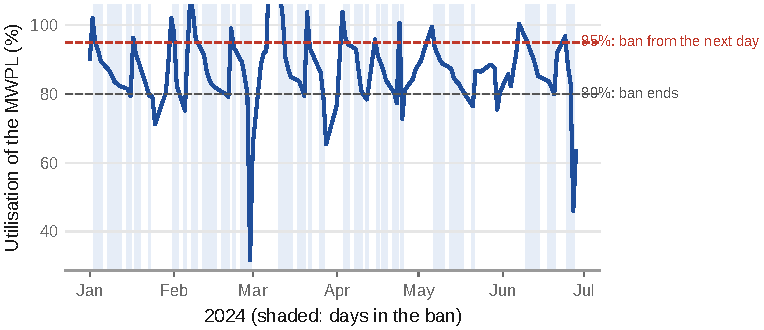
\includegraphics[width=\linewidth]{fig_util_example}
        \caption{Utilisation of the MWPL for SAIL, January to June 2024; shaded: ban days.}
      \end{figure}
    \end{column}
  \end{columns}
\end{frame}

\begin{frame}{Research question and the two stages}
  \begin{block}{Research question}
    How strongly do limits to arbitrage bind in the Indian equity market, and how much mispricing do they explain?
  \end{block}
  \vspace{2pt}
  \begin{columns}[T]
    \begin{column}{0.5\textwidth}
      \begin{exampleblock}{Stage I (this presentation)}
        \scriptsize
        \begin{enumerate}
          \item A model with every Indian limit as a parameter
          \item A test plan frozen before any outcome was related to any treatment
          \item A data set from public exchange files
          \item How wide is the no-arbitrage band?
          \item Do costs and frictions set its edges?
          \item Does the ban bind on trading?
        \end{enumerate}
      \end{exampleblock}
    \end{column}
    \begin{column}{0.5\textwidth}
      \begin{block}{Stage II}
        \scriptsize
        \begin{enumerate}
          \item What a ban does to the basis
          \item Position limits before a ban
          \item Arbitrage capital and the band
          \item Short-sale access across the market
          \item Policy
        \end{enumerate}
      \end{block}
    \end{column}
  \end{columns}
\end{frame}

\begin{frame}{Research gaps}
  \begin{table}
    \scriptsize
    \caption{Earlier Indian estimates of the futures-cash band}
    \begin{tabular}{@{}p{3.1cm}p{2.5cm}p{2.0cm}p{2.6cm}@{}}
      \toprule
      Study & Sample & Data & Band \\
      \midrule
      Aggarwal (2015) & 141 stocks, 2013 & One-second & $-15$ to $+3$\bp \\
      Shankar, Sankar and Kiran Kumar (2019) & 102 stocks, 2007 to 2009 & Five-minute & $-39$ to $-10$\bp \\
      Slivka, Shah and Wu (2011) & Cost calculation & Fee schedules & Twice mature markets \\
      \textbf{This study} & \textbf{360 stocks, 2015 to 2026} & \textbf{Daily} & $\mathbf{-34.5}$ to $\mathbf{+23.9}$\bp \\
      \bottomrule
    \end{tabular}
  \end{table}
  \begin{itemize}
    \small
    \item Earlier bands are intraday objects over a few months or years; the overnight band, where delivery taxes are
    paid, has not been measured over a long panel.
    \item No study has modelled or tested the F\&O ban.
  \end{itemize}
\end{frame}

\begin{frame}{Contributions of Stage I}
  \begin{enumerate}
    \item A model of arbitrage in which each Indian limit is a parameter, including the ban as a reduce-only rule for
    every participant.
    \item A pre-analysis plan with falsifiers, frozen with a time stamp before the tests.
    \item The no-arbitrage band of Indian stock futures over twelve years of daily data, with threshold and
    smooth-transition models.
    \item A test of whether costs and frictions set the band.
    \item The first evidence on how the F\&O ban affects trading, and how the 2025 rules changed the number of bans.
  \end{enumerate}
\end{frame}

%======================================================================================================================
\section{Background and Literature}

\begin{frame}{Why arbitrage is limited}
  \begin{itemize}
    \item \textbf{Capital:} arbitrageurs invest other people's money; losses bring withdrawals when gaps widen
    (Shleifer and Vishny, 1997).
    \item \textbf{Risk:} noise-trader risk deters arbitrageurs with short horizons (De Long et al., 1990).
    \item \textbf{Costs and short sales:} a shorting cost makes the band around fair value asymmetric; margins make
    capital bind (Gromb and Vayanos, 2010).
    \item \textbf{The band:} threshold models of futures and cash (Dwyer, Locke and Yu, 1996); smooth adjustment when
    arbitrageurs differ (Tse, 2001); costs estimated from the band (Ters and Urban, 2020).
    \item \textbf{India:} intraday bands for stock futures (Aggarwal, 2015; Shankar, Sankar and Kiran Kumar, 2019).
  \end{itemize}
\end{frame}

%======================================================================================================================
\section{Institutional Setting}

\begin{frame}{Dated changes to the limits, 2015 to 2026}
  \begin{figure}
    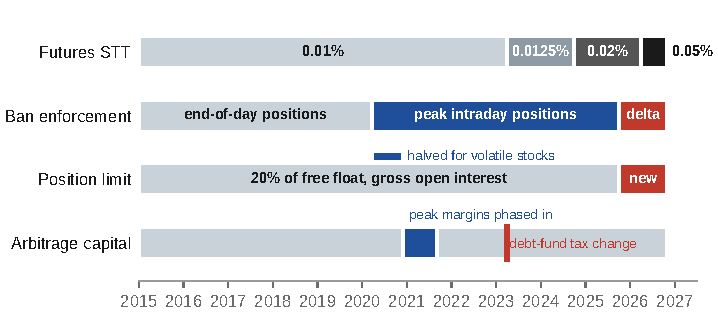
\includegraphics[width=\linewidth]{fig_timeline}
    \caption{Futures STT, enforcement of the ban, the position-limit rule and arbitrage capital.}
  \end{figure}
  \small
  \begin{itemize}
    \item Ban violations were judged on end-of-day positions to 22 March 2020, on peak intraday positions from 23 March
    2020, and on end-of-day delta from October 2025.
  \end{itemize}
\end{frame}

\begin{frame}{Position limits, short selling and costs}
  \begin{table}
    \scriptsize
    \caption{The market-wide position limit over the sample}
    \begin{tabular}{@{}p{2.4cm}p{4.6cm}p{3.2cm}@{}}
      \toprule
      Period & MWPL & Open interest tested \\
      \midrule
      To 30 Sep 2025 & 20\% of free float & Gross, futures and options \\
      Mar to Nov 2020 & Halved for volatile or heavily used stocks & Gross \\
      From 1 Oct 2025 & Lower of 15\% of free float and 65 times average daily delivery; floor 10\% & Delta-adjusted \\
      \bottomrule
    \end{tabular}
  \end{table}
  \begin{itemize}
    \small
    \item Only F\&O stocks may be sold short; naked shorting is barred; stock lending is thin. The practical overnight
    short is a future, so reverse arbitrage is costly.
    \item Futures STT: 0.01\% (2013), 0.0125\% (Apr 2023), 0.02\% (Oct 2024), 0.05\% (Apr 2026); cash delivery pays
    0.1\% on each side.
  \end{itemize}
\end{frame}

%======================================================================================================================
\section{Theoretical Model}

\begin{frame}{Set-up}
  \begin{itemize}
    \item Basis $m=\ln F-\ln F^*$, with $F^*=(S-\mathrm{PV}(D))\,e^{r(T-t)}$.
    \item Outside traders create demand pressure $u$ toward futures; an arbitrage sector holds $a$ units of
    cash-and-carry (long stock, short future). Market clearing:
    \[ m=\frac{u-a}{\Phi}. \]
    \item The sector maximises
    \[ a\,m-\tfrac{\gamma}{2}a^2-c_+a^+-c_-a^-,\qquad \gamma=\alpha\sigma^2, \]
    where $c_+$ is the cost of cash-and-carry and $c_-$ the cost of the reverse trade.
    \item Every Indian limit is a parameter: costs ($c_\pm$), short sales ($c_-$), capital and risk ($\gamma$),
    position limits (the reduce-only rule).
  \end{itemize}
\end{frame}

\begin{frame}{The no-arbitrage band}
  \begin{columns}[c]
    \begin{column}{0.5\textwidth}
      \begin{proposition}[An asymmetric band]
        \small No arbitrage pays while $m$ lies in $[-c_-,\,c_+]$; inside, $m$ follows demand ($\partial m/\partial
        u=1/\Phi$); outside, arbitrage absorbs part of each push ($\gamma/(\gamma\Phi+1)$).
      \end{proposition}
      \begin{proposition}[What moves the band]
        \small Costs set the edges one for one; capital and risk set how far $m$ travels beyond them; the band
        narrows toward expiry and sits below zero when $c_->c_+$.
      \end{proposition}
    \end{column}
    \begin{column}{0.5\textwidth}
      \begin{figure}
        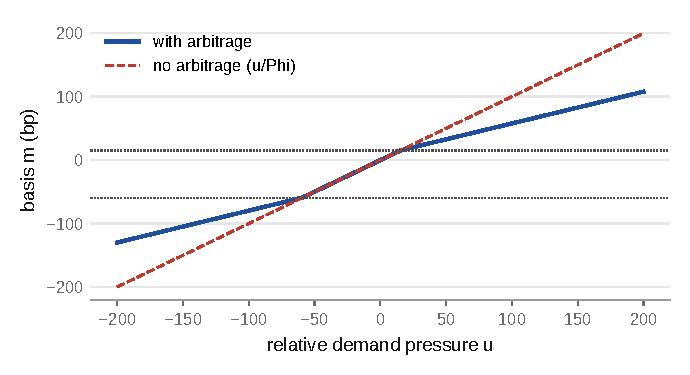
\includegraphics[width=\linewidth]{model_band}
        \caption{Equilibrium basis against demand pressure (illustrative costs).}
      \end{figure}
    \end{column}
  \end{columns}
\end{frame}

\begin{frame}{Existing positions move the band}
  \begin{proposition}[The band moves with the existing book]
    With a position $a_{t-1}$ and an unwinding cost $c_u$, the sector trades only when $m_t$ leaves
    $[\gamma a_{t-1}-c_u,\ \gamma a_{t-1}+c_+]$.
  \end{proposition}
  \vspace{4pt}
  \begin{itemize}
    \item The edges shift with the size of the book, so a fixed-threshold model estimates an \textbf{average} edge,
    not the cost.
    \item Checked on data simulated from the model: with costs of 15\bp\ to add and 10\bp\ to unwind, the estimated
    thresholds were about $-10$ and $0$\bp.
    \item Hence the cost test compares \alert{changes} in the upper edge around tax increases, not its level.
  \end{itemize}
\end{frame}

\begin{frame}{The F\&O ban as a reduce-only rule}
  \begin{assumption}[Ban]
    \small (B1) Arbitrageurs may only reduce: $0\le a_t\le a_{t-1}$. (B2) New futures demand is blocked; a share
    $\chi$ moves to the stock, the rest is withdrawn.
  \end{assumption}
  \begin{proposition}[One-sided correction]
    \small Rich futures are no longer corrected; cheap futures are, while positions last.
  \end{proposition}
  \begin{proposition}[Level effect]
    \small The ban raises the basis when pressure comes from closing trades and lowers it when new demand keeps
    arriving.
  \end{proposition}
  \begin{proposition}[Trading in a ban]
    \small If the rule binds on every trade, each trade closes positions: $\Delta OI=-V$, and futures volume falls.
  \end{proposition}
  {\scriptsize Stage I tests the trading proposition; the price propositions are tested in Stage II.}
\end{frame}

\begin{frame}{A simulated ban}
  \begin{figure}
    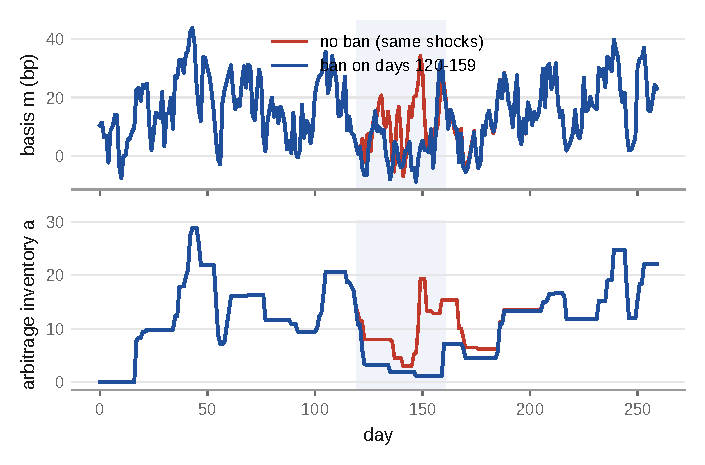
\includegraphics[width=0.82\linewidth]{model_path}
    \caption{Same shocks with and without a ban on days 120 to 159: basis (top) and arbitrage position (bottom).
    Illustrative parameters.}
  \end{figure}
\end{frame}

\begin{frame}{Predictions and falsifiers}
  \begin{table}
    \scriptsize
    \caption{Predictions of the model; primary hypotheses of the test plan in bold}
    \begin{tabular}{@{}p{1.4cm}p{5.1cm}p{2.6cm}p{1.2cm}@{}}
      \toprule
      Label & Prediction & Contradicted if & Stage \\
      \midrule
      Band & The basis moves in an asymmetric band & No band; symmetric & I \\
      \textbf{H3} & Tax increases raise the upper edge & Edges unrelated to costs & I \\
      H1 & Wider bands where frictions are higher & No relation & I \\
      \textbf{H8} & In a ban futures volume falls and $\Delta OI\approx -V$ & Futures activity unchanged & I \\
      \midrule
      \textbf{H7} & In a ban rich futures revert more slowly & No asymmetry & II \\
      Level & The level effect follows the composition of trading & Sign unrelated & II \\
      \textbf{H6} & Short-sale access speeds price adjustment & No change & II \\
      H9, H4, H5, H2 & Anticipation; capital; anomalies; bad news in bans & No relation & II \\
      \bottomrule
    \end{tabular}
  \end{table}
  \footnotesize The four primary hypotheses are corrected jointly (Holm, 5\%); secondary tests are unadjusted.
\end{frame}

%======================================================================================================================
\section{Data and Methodology}

\begin{frame}{Research design}
  \centering
  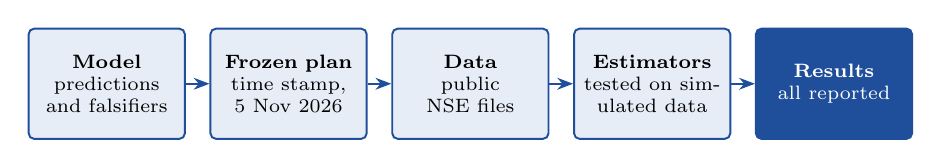
\begin{tikzpicture}[node distance=3mm,
    box/.style={draw=iitbblue,line width=0.7pt,rounded corners=2pt,fill=iitblight,text width=1.75cm,minimum height=1.4cm,align=center,font=\scriptsize},
    arr/.style={-{Stealth[length=2mm]},line width=0.8pt,color=iitbblue}]
    \node[box] (a) {\textbf{Model}\\ predictions and falsifiers};
    \node[box,right=of a] (b) {\textbf{Frozen plan}\\ time stamp, 5 Nov 2026};
    \node[box,right=of b] (c) {\textbf{Data}\\ public NSE files};
    \node[box,right=of c] (d) {\textbf{Estimators}\\ tested on simulated data};
    \node[box,right=of d,fill=iitbblue,text=white] (e) {\textbf{Results}\\ all reported};
    \foreach \x/\y in {a/b,b/c,c/d,d/e} \draw[arr] (\x) -- (\y);
  \end{tikzpicture}
  \vspace{8pt}
  \begin{itemize}
    \small
    \item \textbf{Methods in Stage I:} three-regime threshold and smooth-transition models; event comparisons with
    placebo dates; two-way fixed effects with clustered errors; density test and regression discontinuity at 95\%.
    \item Every detail the plan left open was fixed in a dated log before the test that needed it.
  \end{itemize}
\end{frame}

\begin{frame}{Data}
  \begin{table}
    \scriptsize
    \caption{Public data sources}
    \begin{tabular}{@{}p{3.6cm}p{4.6cm}p{2.0cm}@{}}
      \toprule
      Source & Content & Coverage \\
      \midrule
      NSE open interest, ban lists & MWPL, open interest, ban status & 2010 to 2026 \\
      NSE bhavcopies, delivery files & Futures and cash prices, volumes, delivery & 2015 to 2026 \\
      NSE corporate actions & Dividends and other events & 2014 to 2026 \\
      NSE securities lending & Daily lending trades & 2015 to 2026 \\
      OECD via FRED & Three-month interbank rate & 2011 to 2026 \\
      \bottomrule
    \end{tabular}
  \end{table}
  \begin{exampleblock}{Checks}
    \small Next-day flags match the official ban list for 11,753 of 11,764 flags; the 95\% and 80\% rules hold for 99.4\%
    and 99.7\% of spells; a full rerun reproduces every number.
  \end{exampleblock}
\end{frame}

\begin{frame}{The futures-cash basis}
  \[ m_{it}=\ln\bar F_{it}-\ln\big(\bar S_{it}-\mathrm{PV}_{it}(D)\big)-r_t\tau_{it} \]
  \vspace{-6pt}
  \begin{columns}[c]
    \begin{column}{0.4\textwidth}
      \scriptsize
      \begin{itemize}
        \item Volume-weighted prices, not settlement prices (set at cost of carry on thin days)
        \item Near-month contract, at least 5 contracts, no dividend in its life
        \item 486,040 stock-days, 371 stocks
        \item Median $+1.1$\bp; 10th and 90th percentiles $-39.1$ and $+26.8$\bp
      \end{itemize}
    \end{column}
    \begin{column}{0.6\textwidth}
      \begin{figure}
        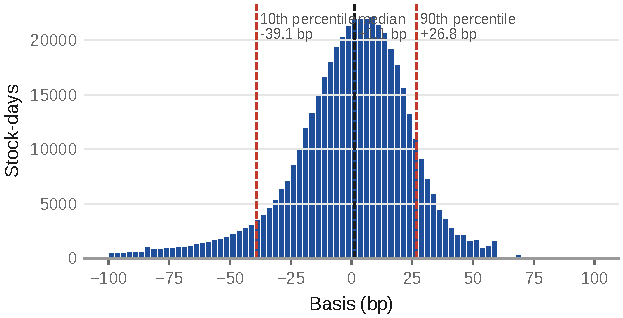
\includegraphics[width=\linewidth]{fig_basis_dist}
        \caption{Distribution of the basis (bp).}
      \end{figure}
    \end{column}
  \end{columns}
\end{frame}

\begin{frame}{Bans over time}
  \begin{figure}
    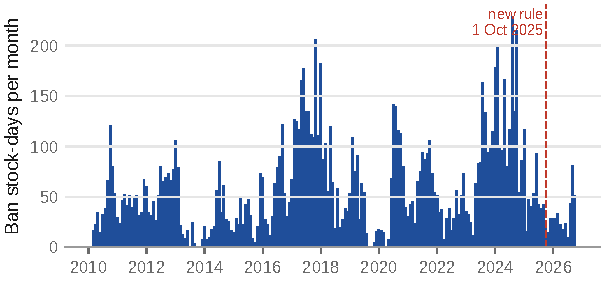
\includegraphics[width=0.92\linewidth]{fig_ban_month}
    \caption{Stock-days in the ban per month, 2010 to 2026.}
  \end{figure}
  \footnotesize
  \begin{itemize}
    \item 1,788 spells, 9,416 stock-days, 141 stocks (2015 to October 2026); a typical spell lasted 4 trading days
    before the reform and 9 after it.
  \end{itemize}
\end{frame}

%======================================================================================================================
\section{Results I: The No-Arbitrage Band}

\begin{frame}{A three-regime threshold model}
  \[
  \Delta m_t=a_r+\rho_r\,x_{t-1}+e_t,\qquad
  r=\begin{cases}\text{lower} & x_{t-1}<g_L\\ \text{middle} & g_L\le x_{t-1}\le g_U\\ \text{upper} & x_{t-1}>g_U\end{cases}
  \]
  \begin{itemize}
    \small
    \item $x_{t-1}$: yesterday's basis minus the stock's median on non-ban days; $\Delta m_t$: change of the same
    contract.
    \item Thresholds by least squares over a grid of percentiles (at least 10\% in each outer regime).
    \item Linearity tested with a sup-$F$ statistic and a wild bootstrap clustered by day; threshold intervals by
    resampling whole stocks.
    \item Prediction: $\rho$ near zero inside the band, clearly negative outside.
  \end{itemize}
\end{frame}

\begin{frame}{The basis moves in a wide, asymmetric band}
  \begin{columns}[c]
    \begin{column}{0.5\textwidth}
      \begin{figure}
        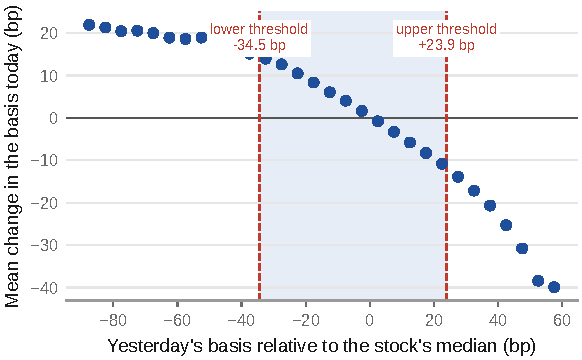
\includegraphics[width=\linewidth]{fig_band_scatter}
        \caption{Mean daily change by yesterday's deviation.}
      \end{figure}
    \end{column}
    \begin{column}{0.5\textwidth}
      \begin{table}
        \scriptsize
        \caption{Pooled threshold model, 473,110 obs.}
        \begin{tabular}{lccc}
          \toprule
          & Lower & Middle & Upper \\
          \midrule
          Threshold & $-34.5$ & & $+23.9$ \\
          Share & 0.12 & 0.76 & 0.12 \\
          Slope & $-0.084$ & $-0.468$ & $-0.809$ \\
          IV slope & $-0.121$ & $-0.192$ & $-0.141$ \\
          \bottomrule
        \end{tabular}
      \end{table}
      \scriptsize Linearity rejected (sup-$F$ 7,471, critical value 31). The lower edge is further away, as expected
      when the reverse trade is costlier.
    \end{column}
  \end{columns}
\end{frame}

\begin{frame}{Noise, smooth adjustment and stability}
  \begin{columns}[c]
    \begin{column}{0.45\textwidth}
      \footnotesize
      \begin{itemize}
        \item \textbf{Noise:} measurement error biases slopes toward $-1$; instrumenting $x_{t-1}$ with $x_{t-2}$
        shrinks all three slopes. Where the band lies is robust; how fast the basis returns is not.
        \item \textbf{Smooth transition:} a logistic model fits almost as well as the threshold model; a symmetric
        exponential one fits worse.
        \item \textbf{Expiry:} lower edge $-40$\bp\ far from expiry, $-28$\bp\ in the last ten days.
      \end{itemize}
    \end{column}
    \begin{column}{0.55\textwidth}
      \begin{figure}
        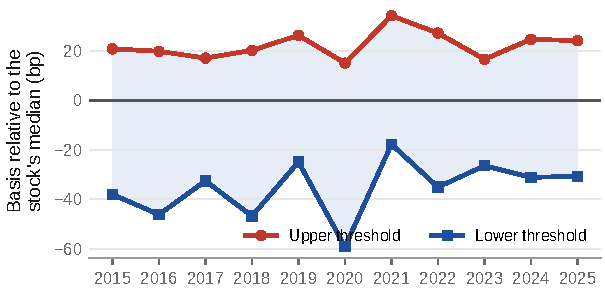
\includegraphics[width=\linewidth]{fig_band_years}
        \caption{Thresholds by year, 2015 to 2025.}
      \end{figure}
    \end{column}
  \end{columns}
\end{frame}

%======================================================================================================================
\section{Results II: What Sets the Band}

\begin{frame}{Tax increases and the upper edge (H3)}
  \begin{figure}
    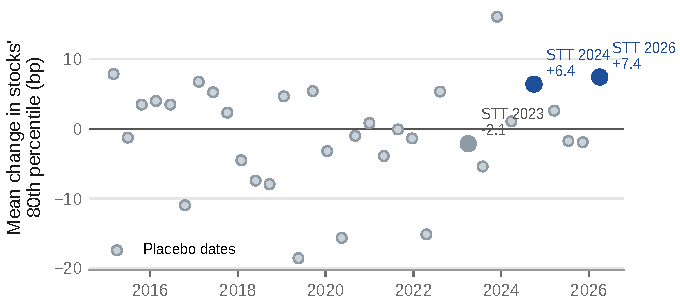
\includegraphics[width=0.78\linewidth]{fig_h3_placebo}
    \caption{Mean change in stocks' 80th percentile of the basis at the STT dates and at 30 placebo dates (bp).}
  \end{figure}
  \footnotesize
  \begin{itemize}
    \item Pre-specified: $+6.96$\bp\ (s.e.\ 0.61) pooling 2024 and 2026; ordered as the cost changes. Supported, and
    significant after Holm.
    \item But the rises exceed the cost changes, the median moved too, and placebo dates move as much (s.d.\ 7.4\bp).
  \end{itemize}
\end{frame}

\begin{frame}{The cost of a new cash-and-carry position}
  \begin{figure}
    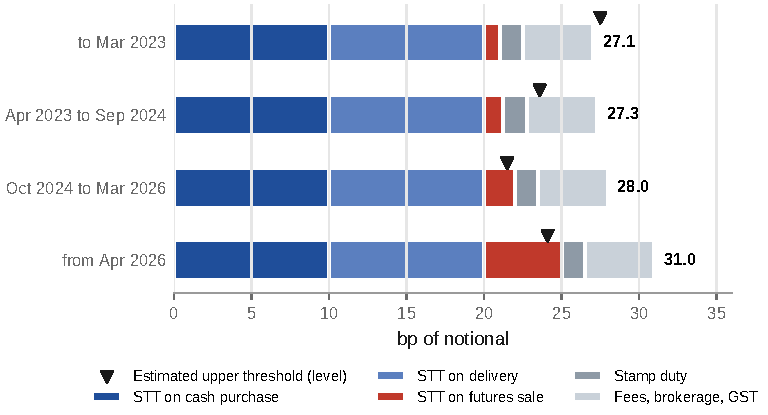
\includegraphics[width=0.8\linewidth]{fig_cost_band}
    \caption{Round trip of an overnight position held to delivery, by STT period (bp of notional).}
  \end{figure}
  \footnotesize
  \begin{itemize}
    \item A new round trip costs 27 to 31\bp, above the estimated upper edge (+22 to +28\bp); rolling costs 4 to 8\bp.
    \item New capital enters only at large gaps; funds that roll lean against small ones.
  \end{itemize}
\end{frame}

\begin{frame}{Frictions across stocks (H1)}
  \begin{figure}
    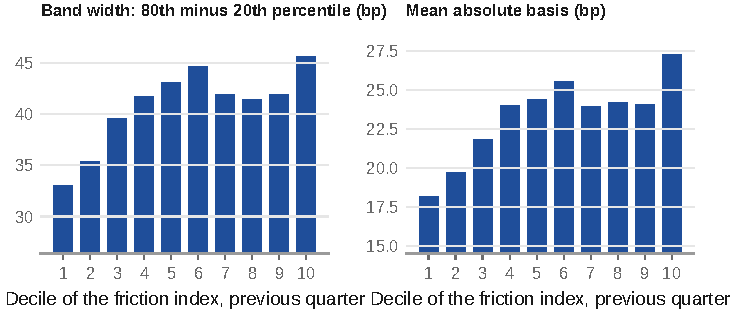
\includegraphics[width=0.86\linewidth]{fig_h1_bins}
    \caption{Band width and mean absolute basis by decile of a friction index of the previous quarter.}
  \end{figure}
  \footnotesize
  \begin{itemize}
    \item Index: spread, illiquidity, idiosyncratic volatility, utilisation, lack of stock lending. One s.d.\ more:
    band $+3.5$\bp\ (s.e.\ 1.1, $p=0.002$), mean width 40.8\bp.
    \item Across stocks only: with stock fixed effects the relation disappears.
  \end{itemize}
\end{frame}

%======================================================================================================================
\section{Results III: Does the Ban Bind on Trading?}

\begin{frame}{Trading in a ban (H8)}
  \[ y_{it}=\beta\,\mathrm{Ban}_{it}+\alpha_{i,b(\omega_{i,t-1})}+\lambda_t+\varepsilon_{it} \]
  \vspace{-8pt}
  \begin{table}
    \scriptsize
    \caption{Ban days against the same stock's non-ban days at 80 to 95\% utilisation, 2015 to September 2025}
    \begin{tabular}{lcc}
      \toprule
      Outcome & Effect (s.e.) & Non-ban mean \\
      \midrule
      log(1 + futures contracts) & $-2.00$ (0.11) & 8.50 \\
      log(1 + cash shares) & $+0.073$ (0.027) & 15.80 \\
      Delivery share & $+0.041$ (0.005) & 0.26 \\
      \bottomrule
    \end{tabular}
  \end{table}
  \begin{itemize}
    \footnotesize
    \item Futures trading falls by about 87\%; cash trading rises and moves toward delivery. Supported, and
    significant after Holm.
  \end{itemize}
\end{frame}

\begin{frame}{Enforcement decides whether the rule binds}
  \begin{figure}
    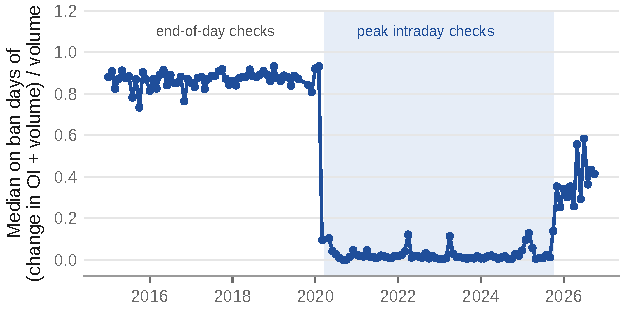
\includegraphics[width=0.85\linewidth]{fig_ban_R}
    \caption{Monthly median of $R=(\Delta OI+V)/V$ on ban days; $R=0$ when every trade closes a long and a short.}
  \end{figure}
  \footnotesize
  \begin{itemize}
    \item End-of-day checks (to 22 March 2020): median 0.87. Peak intraday checks: 0.011. Delta rule (from October
    2025): 0.19 to 0.36. Futures effect $-0.97$ vs $-2.72$ log points.
  \end{itemize}
\end{frame}

\begin{frame}{The 95\% trigger}
  \begin{columns}[c]
    \begin{column}{0.5\textwidth}
      \begin{figure}
        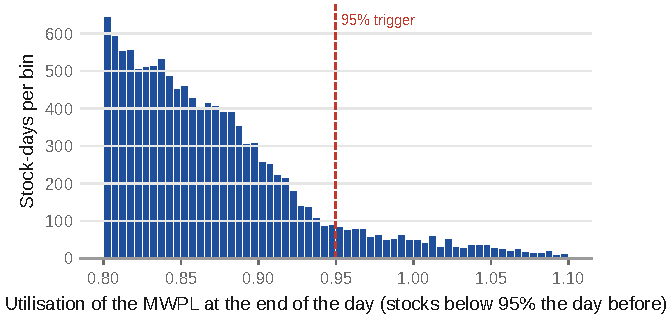
\includegraphics[width=\linewidth]{fig_density}
        \caption{Utilisation of stocks below 95\% the day before.}
      \end{figure}
      \scriptsize No bunching: $T=-0.18$, $p=0.86$. The chance of crossing next day rises from 7\% at 85\% to about
      half at 93 to 95\%.
    \end{column}
    \begin{column}{0.5\textwidth}
      \begin{figure}
        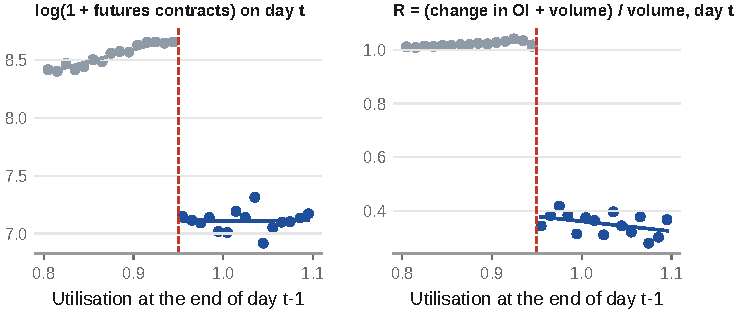
\includegraphics[width=\linewidth]{fig_rd_trading}
        \caption{Futures contracts and $R$ around 95\%.}
      \end{figure}
      \scriptsize Futures $-1.53$ log points, $R$ $-0.66$, delivery share $+5.1$ points; cash volume no jump.
    \end{column}
  \end{columns}
\end{frame}

\begin{frame}{The 2025 rules and ``spurious'' bans}
  \begin{figure}
    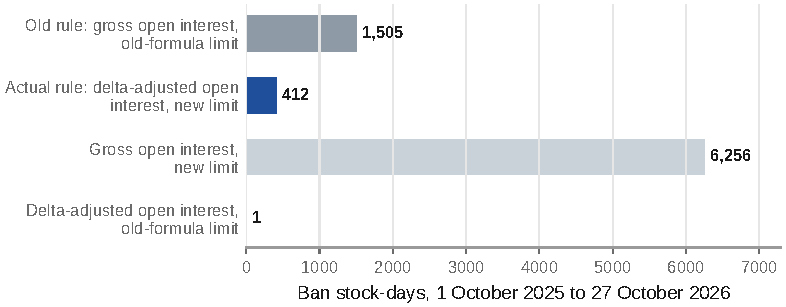
\includegraphics[width=0.78\linewidth]{fig_spurious}
    \caption{Ban stock-days, 1 October 2025 to 27 October 2026, under the actual and three counterfactual rules.}
  \end{figure}
  \footnotesize
  \begin{itemize}
    \item Before 2025 bans came from rising open interest: only 0.4\% of entries were caused by a falling limit.
    \item Delta-adjusted open interest removes almost all bans; the lower limit alone would have quadrupled them. Net:
    412 ban days against 1,505 under the old rule.
  \end{itemize}
\end{frame}

%======================================================================================================================
\section{Conclusions and Stage II}

\begin{frame}{Summary of the Stage I tests}
  \begin{table}
    \scriptsize
    \caption{Pre-specified tests of Stage I}
    \begin{tabular}{@{}p{3.0cm}p{2.9cm}p{4.3cm}@{}}
      \toprule
      Test & Result & Comment \\
      \midrule
      \textbf{H8} trading in a ban & Supported ($p<10^{-10}$) & Every trade closes positions under intraday checks \\
      \textbf{H3} costs and the band & Supported ($p<10^{-10}$) & Weak against placebo dates; a common shift \\
      H1 frictions and the band & $p=0.002$ & Across stocks only \\
      Density at 95\% & $p=0.86$ & No bunching \\
      Band estimation & sup-$F$ 7,471 & $-34.5$ to $+23.9$\bp; stable over time \\
      \bottomrule
    \end{tabular}
  \end{table}
  \footnotesize Primary tests (bold) Holm-corrected with the two primary tests of Stage II.
\end{frame}

\begin{frame}{Conclusions}
  \begin{itemize}
    \item The basis of Indian stock futures moves in a \textbf{wide, asymmetric band}, about $-35$ to $+24$\bp\
    around each stock's median, much wider than intraday bands.
    \item \textbf{Costs shape the band loosely}: a new position costs 27 to 31\bp, in the outer tail; the upper edge
    rose after tax increases, but not unusually.
    \item \textbf{Frictions} widen the band across stocks.
    \item \textbf{The ban binds hard on trading}: futures volume $-87\%$; every trade closes positions once checks are
    intraday. Enforcement matters as much as the rule.
    \item The 2025 rules cut ban days by about \textbf{three quarters}.
  \end{itemize}
\end{frame}

\begin{frame}{Limitations and Stage II}
  \begin{columns}[T]
    \begin{column}{0.5\textwidth}
      \begin{alertblock}{Limitations}
        \scriptsize
        \begin{itemize}
          \item Daily data: noise inflates measured reversion
          \item Arbitrage positions are not observed
          \item Three tax events, one confounded
          \item Only 44 ban spells since October 2025
        \end{itemize}
      \end{alertblock}
    \end{column}
    \begin{column}{0.5\textwidth}
      \begin{exampleblock}{Stage II}
        \scriptsize
        \begin{itemize}
          \item The ban and the basis: one-sided correction (H7), the level at ban start, placebo bans
          \item Position limits before a ban; the 2020 halving
          \item Arbitrage capital and the band
          \item Short-sale access: F\&O entry (H6), anomalies, a constraint index
          \item Policy on position limits
        \end{itemize}
      \end{exampleblock}
    \end{column}
  \end{columns}
\end{frame}

\begin{frame}[allowframebreaks]{Important references}
  \tiny
  \begin{thebibliography}{99}
    \bibitem{agg} Aggarwal, N. (2015). Limits to arbitrage: The case of single stock futures and spot prices. IGIDR WP-2015-010.
    \bibitem{cjm} Cattaneo, M., M. Jansson and X. Ma (2020). Simple local polynomial density estimators. \emph{J. American Statistical Association} 115(531).
    \bibitem{dssw} De Long, J. B., A. Shleifer, L. Summers and R. Waldmann (1990). Noise trader risk in financial markets. \emph{J. Political Economy} 98(4).
    \bibitem{dly} Dwyer, G., P. Locke and W. Yu (1996). Index arbitrage and nonlinear dynamics between the S\&P 500 futures and cash. \emph{Rev. Financial Studies} 9(1).
    \bibitem{gv} Gromb, D. and D. Vayanos (2010). Limits of arbitrage. \emph{Annual Rev. Financial Economics} 2.
    \bibitem{kp} Kolari, J. and S. Pynn\"onen (2010). Event study testing with cross-sectional correlation of abnormal returns. \emph{Rev. Financial Studies} 23(11).
    \bibitem{sebi} SEBI (2025). Circular SEBI/HO/MRD/TPD-1/P/CIR/2025/79; NSE Clearing circular 119/2025.
    \bibitem{ssk} Shankar, R. L., G. Sankar and K. Kiran Kumar (2019). Mispricing in single stock futures: Empirical examination of Indian markets. \emph{Emerging Markets Finance and Trade} 55(7).
    \bibitem{sv} Shleifer, A. and R. Vishny (1997). The limits of arbitrage. \emph{J. Finance} 52(1).
    \bibitem{ssw} Slivka, R., V. Shah and J. Wu (2011). Arbitrage of single stocks versus futures in India. Working paper.
    \bibitem{tu} Ters, K. and J. Urban (2020). Estimating unknown arbitrage costs: Evidence from a 3-regime threshold vector error correction model. \emph{J. Financial Markets} 47.
    \bibitem{tse} Tse, Y. (2001). Index arbitrage with heterogeneous investors: A smooth transition error-correction analysis. \emph{J. Banking and Finance} 25(10).
  \end{thebibliography}
\end{frame}

\begin{frame}{Acknowledgement}
  I thank my supervisor, Prof.\ Aditi Chaubal, for her guidance throughout this project, and in particular for the
  advice to build a formal model of what the project would test before looking at any data.
\end{frame}

\begin{frame}
  \centering
  {\Huge\color{iitbblue} Thank You}\\[12pt]
  {\small Questions and comments are welcome}
\end{frame}

%======================================================================================================================
\appendix
\section*{Backup Slides}

\begin{frame}{Backup: the propositions and the tests}
  \begin{table}
    \scriptsize
    \begin{tabular}{@{}p{2.6cm}p{5.6cm}p{2.0cm}@{}}
      \toprule
      Proposition & Statement & Tested in \\
      \midrule
      1 Band & Arbitrage only outside $[-c_-,c_+]$ & Stage I \\
      2 What moves it & Costs set the edges; capital the passthrough & Stage I (H3), II (H4) \\
      3 Existing book & The no-trade region moves with the position & Design of H3 \\
      4 One-sided & In a ban rich futures are not corrected & Stage II (H7) \\
      5 Level effect & The ban's effect on the level has no fixed sign & Stage II \\
      6 Trading & Each trade in a ban closes positions: $\Delta OI=-V$ & Stage I (H8) \\
      \bottomrule
    \end{tabular}
  \end{table}
  \footnotesize Proofs are in the appendix of the Stage I report.
\end{frame}

\begin{frame}{Backup: the basis and time to expiry}
  \begin{figure}
    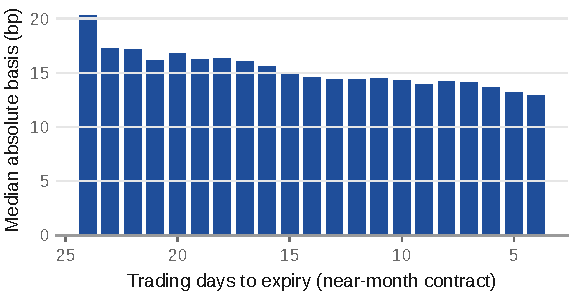
\includegraphics[width=0.85\linewidth]{fig_basis_expiry}
    \caption{Median absolute basis of the near-month contract by trading days to expiry.}
  \end{figure}
\end{frame}

\begin{frame}{Backup: the October 2025 cut in the position limit}
  \begin{figure}
    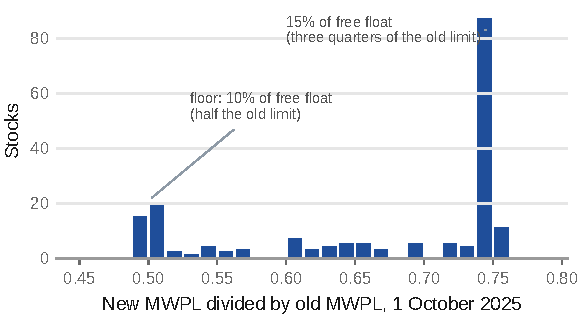
\includegraphics[width=0.9\linewidth]{fig_mwpl_ratio}
    \caption{New MWPL divided by old MWPL, 1 October 2025 (208 stocks).}
  \end{figure}
\end{frame}

\begin{frame}{Backup: the pre-analysis plan and its log}
  \small
  \begin{itemize}
    \item Frozen with a time-stamped tag on 5 November 2026, after the supervisor's go-ahead and a full set of data
    checks; until then no outcome was related to any treatment.
    \item Every detail the plan left open (sample filters, utilisation bins, placebo dates, density population) was
    fixed in a dated log before the test that needed it.
    \item Analyses added after a result (the split by enforcement period, the noise correction) are labelled as such;
    the pre-specified result is reported first.
    \item Each estimator first recovered known effects on simulated data.
  \end{itemize}
\end{frame}

\end{document}
